\chapter{Propuesta}
\hrule \bigskip \vspace*{1cm}
%------------------------------------------------------------------------

% La propuesta es la descripción detallada de las secuencias de etapas, pasos o instrucciones a seguir para lograr demostrar una hipótesis o alcanzar un objetivo planteado. Se debe incluir diagramas que permitan visualizar todo el proceso propuesto para mejorar la comprensión de la idea planteada.
% La propuesta debe responde las siguientes preguntas:
% ¿Cómo se puede lograr el objetivo?
% ¿Cuál es la secuencia de pasos a seguir para lograr alcanzar el objetivo general planteado?
% 	En caso de haber planteado una hipótesis, la propuesta debe demostrar la secuencia de pasos o actividades a ser realizados para verificar si la hipótesis es verdadera o falsa.



\begin{figure}[h]
    \centering
    \includegraphics[width=15cm]{Graficos/Azul y Blanco Diagrama de Flechas Presentación2.png}
    %\caption{Caption}
    \label{fig:enter-label}
\end{figure}


\begin{itemize}
    \item \textbf{Preprocesamiento:}
En esta etapa, se preparan los datos antes de alimentarlos al modelo de aprendizaje automático. Esto puede incluir:
\textbf{Limpieza de datos:}
Utilizando \cite{DERDIYOK2024109896} se eliminar valores atípicos, completar datos faltantes con  interpolación lineal ,eliminar datos inconsistentes .
\textbf{Filtro:} Se aplica un filtro  Butterworth low-pass filter de 5HZ   .
\textbf{Normalización:} Escalar los datos para que tengan una escala similar Min-max scaling.



    \item \textbf{Detección de características:}
Aquí se extraen características relevantes de los datos.
Se usa  técnicas como:
CVxEDA: parar separar los  componente de la señal EDA en  componente tónico y fasico.
También se  extraen las características estadísticas 


    \item \textbf{Entrenamiento y Clasificación:}
\textbf{Se divide los datos } en entrenamiento y prueba  .
En esta etapa,se utiliza dos algoritmos ,Random Forest y  Redes neuronales, también se encuentra los óptimos Hyperparametros con GridSearch. El modelo ajusta sus parámetros para minimizar el error en las predicciones.

    \item \textbf{Análisis:}
Implica analizar la variabilidad de las propiedades estadísticas la diferencias y similitudes de los dataset .

    \item \textbf{Validación:}
Se evalúa el rendimiento del modelo utilizando datos de prueba.

Se utiliza la Validación cruzada para evaluar el rendimiento de manera robusta.
Se utiliza Métricas de evaluación  como precisión, recall,y se compara con otros estudios similares .



\end{itemize}


Por tanto  se propone  el diseño de  un sistema  para la detección de estrés    a partir de datos fisiológicos EDA de baja resolución.
%y realizar el análisis comparativo  de los datos en entornos de laboratorio .  


\subsection*{ DatabaseWork3d}

El conjunto de datos contiene muestras de situaciones de trabajo fatigantes y libres de estrés,proporciona una representación  de varios niveles de estrés. El conjunto de datos se acompaña de metadatos y anotaciones extensas, que facilitan el análisis e interpretación en profundidad. 

Contiene  datos de actividad electrodérmica (EDA), presión volumétrica sanguínea (BVP), temperatura de la piel y acelerómetro (ACC). EDA se muestrea a 4 Hz y abarca aspectos de conductividad de la piel, fásicos y tónicos, que se distinguen por un umbral de aproximadamente 0,05 ms. La temperatura de la piel se registra constantemente a 4 Hz en grados Celsius. 
Los datos de presión arterial se derivan de la señal del pulso de volumen sanguíneo (BVP) de 64 Hz. Los datos del acelerómetro se recopilan a 64 Hz para medir la fuerza gravitacional (g) en las tres dimensiones espaciales (x, y y z). 

Estas señales se capturan utilizando sensores de pulsera Empatica E4 y se aplica una técnica de reducción de resolución(downsampling) para estandarizar las frecuencias, equilibrando un examen fisiológico exhaustivo. 
y seguimiento continuo de la actividad. La opción de reducción de resolución, que reduce todas las entradas a 4 Hz, garantiza un conjunto de datos consistente y efectivamente fusionado.


\begin{figure}[h]
    \centering
    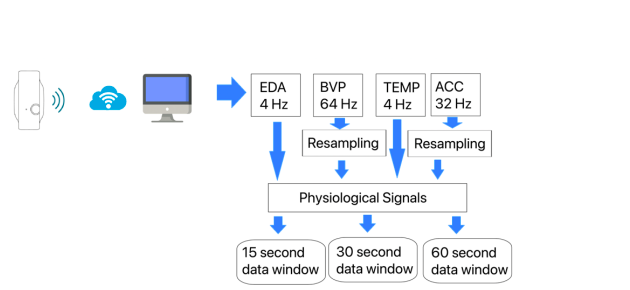
\includegraphics[width=7cm]{Graficos/captura3.png}
    \caption{dataset work3d}
    \label{fig:enter-label}
\end{figure}


\subsection*{Database 2}
Desde un primer momento se utlizara  los conjuntos de datos WESAD, Work3d para probar las hipótesis. Los  conjuntos de datos se utilizan para comparar estadísticamente la precisión de la detección de estrés de los modelos independientes y dependientes del usuario .

Conjunto de datos WESAD: El conjunto de datos publicado consiste en datos fisiológicos recopilados de 15 participantes bajo dos protocolos de estudio diferentes que incluían una combinación de condiciones de diversión/estrés/relajación.




Los archivos del dataset  en su forma natural contienen  información derivada  que en  este estudio se ignoraran : HR.csv, IBI.csv, tags.csv. El archivo info.txt contiene algunos detalles sobre el contenido de la carpeta. Los datos sin procesar del dispositivo E4 están contenidos en los siguientes archivos (en cada archivo, la primera línea se refiere a la marca de tiempo global del canal del sensor al inicio, la segunda línea se refiere a la frecuencia de muestreo del canal del sensor).

\begin{itemize}
    \item ACC.csv: muestreado a 32 Hz. Las 3 columnas de datos se refieren a los 3 canales del acelerómetro. Los datos se proporcionan en unidades de 1/64 g.
    \item BVP.csv: muestreado a 64 Hz. Datos de fotopletismógrafo (PPG).
    \item EDA.csv: muestreado a 4 Hz. Los datos se proporcionan en $\mu$ S.
    \item TEMP.csv: muestreado a 4 Hz. Los datos se proporcionan en grados centigrados .
\end{itemize}

En el experimento ,el dispositivo E4 fue usado en el 
muñeca no dominante de los participantes. La tasa de muestreo de los diferentes sensores fue diferente.
Tambien se registro modalidades de pulso de volumen sanguíneo (BVP) fisiológico de alta resolución, electrocardiograma (ECG), actividad electrodérmica (EDA), electromiograma (EMG), respiración (RESP), temperatura de la piel (TEMP) y movimiento (ACC) con el dispositivo  llamado RespiBAN. Al mismo tiempo, también los participantes usaron la  pulsera Empatica E4 para capturar datos EDA de baja frecuencia de muestreo . 





\subsection{Preprocesamiento}
\begin{figure}
    \centering
    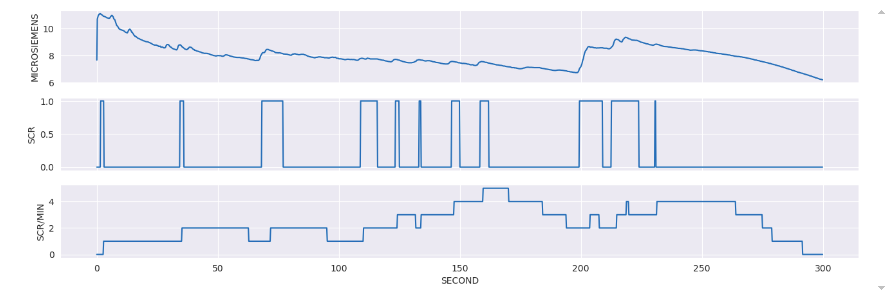
\includegraphics[width=10cm]{Graficos/captura2.png}
    \caption{Caracteristicas}
    \label{fig:enter-label}
\end{figure}


\subsection*{Extracción estadística de características EDA}

La señal EDA se filtró a través de un filtro  Butterworth low-pass filter de cuarto orden de 5 Hz. Lo que significa que sólo la señal EDA de alta resolución de los datos de WESAD-Chest se preprocesa a través de  el filtro  antes de extraer las características . A continuación se extrajeron las características de Eda QUE comprender la respuesta de conducción cutánea (SCR ),nivel de conducción cutánea ,los picos de scr, inicios scr ,y la amplitud scr. junto con  las características estadísticas .El tamaño de ventana y el desplazamiento de ventana fueron de 60 segundos y 30 segundos respectivamente lo que significa que  el modelo busca patrones de estrés después de cada 30 segundos mediante la observación de características estadísticas extraídas  en el paso anterior  en el intervalo de 60 segundos.


\subsection{Entrenamiento}

Utilizando las características estadísticas, se entreno  un modelos de aprendizaje automatico para detectar  estrés : RAndom Forest (RF),y multi- Perceptrón de capa (MLP), utilizando Grid Search .La estandarización de la característica  se aplica para la entrada de MLP, ya que el  modelo funcionan mejor  con datos estandarizados.
Se realizo la estrategia Leave-One-Group-Out (LOGO) para el modelo de detección de estrés independiente del usuario.
 Los datos de entrenamiento y prueba para el entrenamiento dependiente del usuario se dividen mediante   stratified train-test split strategy  (entrenamiento y prueba) cuyo tamaño de prueba es igual al 28,6 \%



\begin{table}[h!]
  \centering
  \caption{Configuraciones de Grid Search de cinco modelos de Aprendizaje Automático utilizados al entrenar modelos de detección de estrés.}
  \label{tab:GridSearchConfiguration}
  \begin{tabular}{|c|c|c|}
    \hline
    \textbf{Modelo} & \textbf{Parámetros GridCV} & \textbf{Valores} \\
  
    \hline
    RF & n\_estimadores & 500, 1000 \\
    & Mínimo de muestras para dividir & 2, 4 \\
    & Mínimo de muestras por hoja & 1, 4 \\
    & Peso de clase & Ninguno, balance \\
    \hline
    MLP & Tamaños de capas ocultas & 64, 128, 256, 512 \\
    \hline
  
  \end{tabular}
\end{table}




\subsection{Análisis}

Lo que se espera es que el modelo dependiente del usuario detecte estadísticamente patrones con mayor precisión que un modelo  independiente del usuario,independientemente  de la elección del modelo de aprendizaje automático.
Se entrenaron 2 modelos independientes y 2 modelos dependientes  configurando LOGO junto con  GridsearH,la métrica  BA son calculados para cada individuo en cada Dataset para crear puntuaciones de evaluación de los modelos independientes y dependientes del usuario respectivamente.
Los datos contienen 2x2(número de modelos)x35 observaciones para ambas salidas ,modelos dependientes y independientes del usuario.
Cada uno consta de resultados independientes  de 2 modelos de aprendizaje automático x35 datos de participantes en 2 conjuntos de datos .

En el  experimentos, nos  enfocamos  en cubrir el análisis usando  estadística inferencial,sobre la población utilizando  un número de  muestras representativas. Se utiliza , la prueba de hipótesis  para estimar el desempeño estadístico de los modelos de detección de estrés  independientes y dependientes del usuario.

 A partir de este punto, las hipótesis nula y alternativa de la prueba unilateral de suma de rangos se 
establecen de la siguiente manera:
\begin{itemize}
    \item  H0 : M1 = M2 (El modelo dependiente del usuario no mejora en distinguir patrones estresantes y no estresantes).
    \item Ha : M1 > M2 (El modelo dependiente del usuario logra distinguir patrones de estrés/no estrés
 de forma  más precisa que uno independiente del usuario).
\end{itemize}

donde , M1 y M2 indican la mediana de las puntuaciones de precisión de la predicción 
de estrés/sin estrés de los modelos dependientes e independientes del usuario.






